\section{Recovery of periods from {\harps} data}
\protect\label{section:harpsper}

After deriving the various measures described in \ref{section:linemeas}, attempts were made to derive periodograms, on
the basis that the ``correct'' result was 82.6 days. As discussed in Appendix \ref{chapter:lsroutines}, all the routines
tried gave different results for all the measures. The {\numrecs} routine, which does not allow easy selection of trial
periods, usually did not find other than short periods of under 10 days. On the rare occasions where longer periods were
found, the reported FAP was 1.0 or very close.

As a result the three Python routines were used and the results compared. The periodograms were all ``noise like'' under
about 40 days, so that had to be selected as a lower limit. For similar reasons 130 days had to be selected as an upper
limit. This encompassed the 41.3 days of \citet{benedict93}, although this looks very likely to be a half-period alias,
through to the 116.6 days of \citet[Table 3]{suarezmascareno15}.
Periodograms were generated for periods between 40 days and 130 days, in steps of 0.01 days (14 minutes, 20 seconds)
taking into account the 41.3 days of \citet{benedict93}, the minimum period of 50 days given by \citet{kurster99}, the
82 days of \citealt{benedict92,benedict98,kiraga07} and the 116.6 days of Many of
the routines reported a plethora of strong shorter periods down to 0.01 days, but these were discounted these for the
purposes of this study, given that the main concern was the rotation period and not other much shorter periodic
behaviour. The erratic behaviour of the periodograms below about 40 days make it impractical to extend the search down
to include the 31.5 days of \citet{guinan96}. Many of the periodograms showed several strong peaks all over the range
searched, with periods reported by others the fourth or fifth strongest peak, so the tables below show the 5 strongest
peaks in all cases. Listed below are results from all the methods described in Sections \ref{section:linemeas} and
\ref{section:alternativelines} with combinations where appropriate.

\subsection{Equivalent Width measurements}
\protect\label{section:ewper}

{\FirstP} computed periodograms from the results for the measures described above in \ref{section:linemeas} using all
three Lomb-Scargle routines and some results are exhibited in Fig. \ref{fig:harpspgrams1}. Unlike with the {\asas}
photometry data, the three routines did not yield consistent results. The main results are summarised in Appendix \ref{chapter:pgramdetail}. In the first two panels of Fig. \ref{fig:harpspgrams1} are shown the periodograms for the
Equivalent Widths and Peak Ratios respectively, processed by {\gatspy}. In the bottom panel of
Fig. \ref{fig:harpspgrams1} is shown the Peak Ratio results after binning to 1 day, showing a returned period close to
82.6 days. It was noticeable that the Equivalent Width and {\ha} Index measures delivered almost identical results in
most cases, particularly with the {\gatspy} routine.


\begin{figure}[!htbp]
\begin{center}
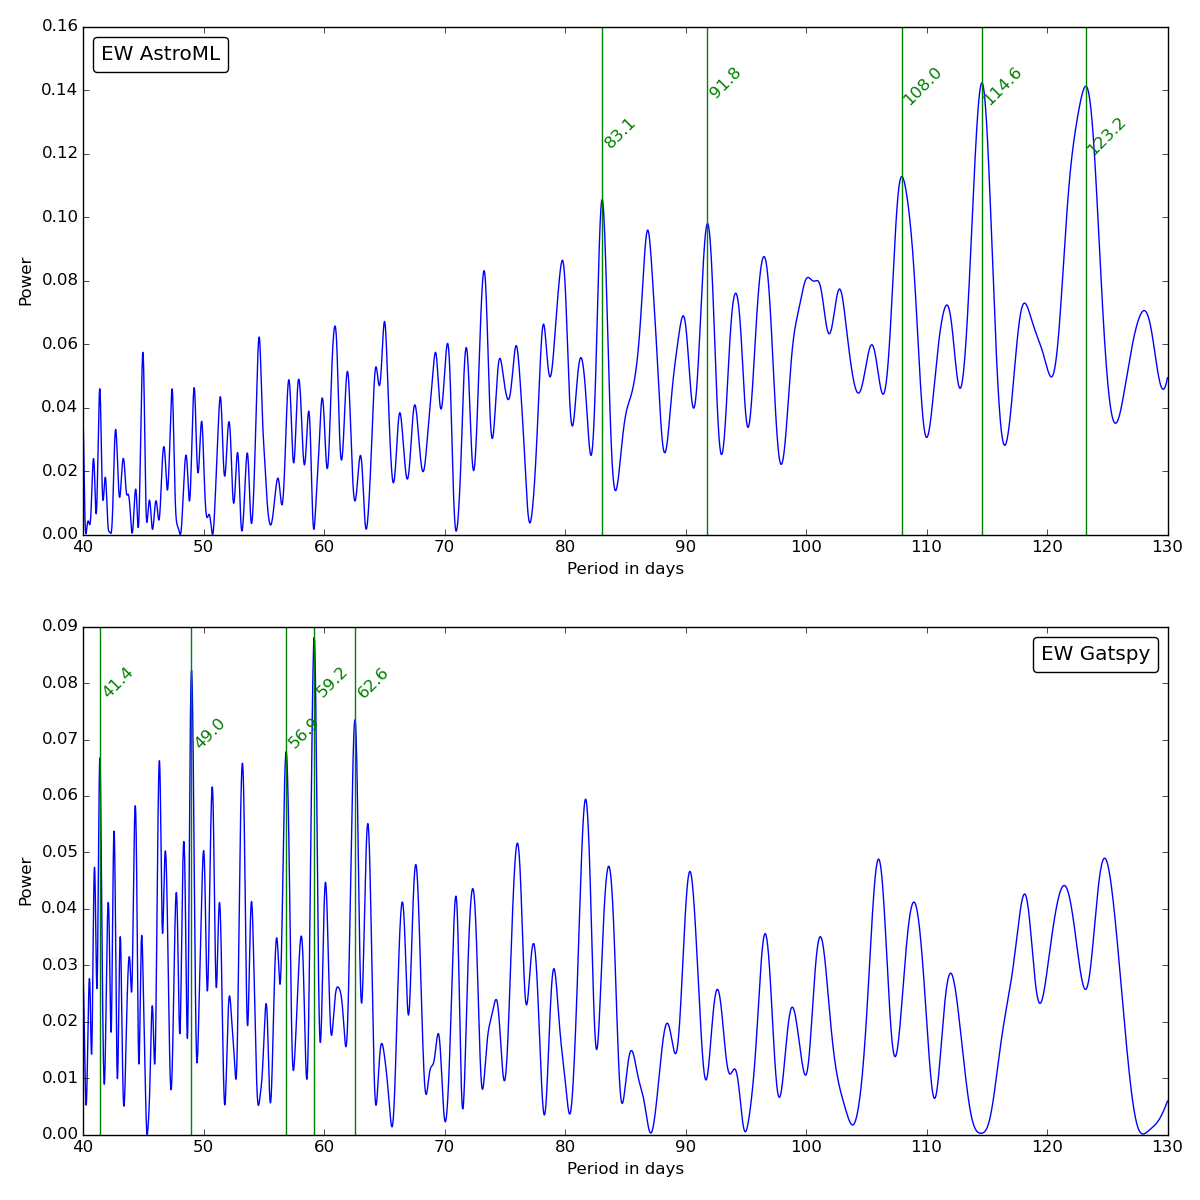
\includegraphics[scale=0.18]{Figures/summpgrams.png} \\
\end{center}   
\caption{This figure shows sample periodograms from the {\ha} peak of the {\harps} data, for the range between 40 days
  and 130 days in steps of 0.01 days. All were made using the {\gatspy} routine.  The top panel shows the periodogram
  derived from the Equivalent Widths (EW) and the middle and bottom panels ones derived from the Peak Ratios (PR). None
  have any clipping of data but the bottom panel is binned to 1 day.  The strongest five peaks are marked on the top two
  panels and the strongest peak of 82.2 days is marked on the bottom panel with the vertical lines.  The results are set
  out more fully in Table \ref{table:peak5compall}.}
\protect\label{fig:harpspgrams1}
\end{figure}

\subsection{{\ha} Index Measurements}
\protect\label{section:haiper}

\subsection{Peak Ratio Measurements}
\protect\label{section:priper}

\subsection{Periods from Residual spectra}
\protect\label{section:residualper}

\subsection{Skewness and Kurtosis measurements}
\protect\label{section:skewkurtper}

\subsection{TiO line and combined lines}
\protect\label{section:tioper}

{\FirstP} considered various other treatments of the data prior to obtaining periodograms. One treatment was to obtain
periodograms of the Equivalent Width and Peak Ratios from the residual spectra after division by the line with the
lowest equivalent width and also the mean of the lowest five spectra. These spectra were ones timed at 5 April 2011 UTC
03:26:33 (the lowest), 16 March 2006 UTC 06:37:59, 14 March 2007 UTC 07:28:29, 8 April 2011 UTC 06:28:17 and 22 April
2011 UTC 05:07:46. {\FirstP} also examined periodograms from the skewness and, following \citet{flores16},
the kurtosis of the {\ha} peaks before and after clipping and binning. However neither of these measurements proved
materially different from the other measurements. It was again possible to reproduce the 116-day period of
\citet{suarezmascareno15} from both the skewness and kurtosis measures.

The periodograms obtained from the {\ha} measurements on the {\harps} data showed a large number of ``beat''
frequencies. They were taken over 11 years from 2004 to 2014 inclusive, however the bulk of these, 207 out of 260, were
in 2013 and 2014. It seemed possible if other periodic behaviour was selectively affecting {\ha} as opposed to the
overall intensity as obtained by \asas, restriction to just the two years might eliminate this. However, on trying this
did not materially affect the quality of the results from these measurements, although the ``beat'' frequencies were
reduced somewhat. It was noticeable, however that all the measurements failed to reproduce the 116-day period after a
different set of observation times was taken, either by selecting only 2013-4 data or by adding in additional
observational data taken in 2016.

The periodograms obtained for all the methods were similar in general appearance to those in Fig. \ref{fig:harpspgrams1}
but all with different peaks, apart from the Equivalent Width measure being generally similar to the {\ha} Index as
Table \ref{table:peak5compall} makes clear. Periods close to the {\asas} or {\hst} results appear more often with the
Peak Ratio measure, otherwise it was noticeable that periods of around 41 days were revealed in a few places,
particularly frequently for Peak Ratio. It can be seen that 116.3 days, as found by \citet{suarezmascareno15}, are
observed in the Equivalent Width and {\ha} Index measure.

In an attempt to remove data contaminated from flares, {\Firstp} clipped spectra with various upper bounds of Equivalent
Width. As discussed in Section \ref{section:uvesflares}, {\Firstp} decided to select the spectra with the lower 90\% of
the Equivalent Widths (i.e. removing the 10\% of profiles containing the highest EWs), which was approximately a maximum
of 1 standard deviation from the median in both the {\harps} and {\uves} data, eliminating the upper 23 spectra from the
{\harps} data. This was then binned to 1 day, giving a net 55 observation dates. This led to a significant improvement
in the results particularly from the Peak Ratio measure, as illustrated in the last panel of Fig. \ref{fig:harpspgrams1}
(although that is binned and not clipped) however no particular improvement was noted in the other measures.  {\FirstP}
also considered eliminating two very isolated epochs of 25 July 2005 at 23:43:51 and 14 March 2007 at 07:28:29, in case
these contained contaminating periodic data, but this made no discernible difference to the results. {\FirstP} also
calculated results for the {\ha} Index but again found the results to be virtually indistinguishable from the Equivalent
Width results after this process.

Again as with the {\asas} and {\hst} data, {\Firstp} checked for other periodic signals of up to the span of the data,
but were unable to discern any strong period and in particular no sign of the 442-day period reported in
\citet{cincunegui07}.
